% Chapter 2

\chapter{Implémentation} % Main chapter title

\label{Chapter2} % For referencing the chapter elsewhere, use \ref{Chapter1}

  
\section{Processus de calibrage}

Comme nous l'avons expliqué dans le chapitre 1, le calibrage de notre caméra va nous permettre d'estimer les différents paramètres de celle-çi afin d'avoir des mesures précises. Ce calibrage va nous permettre de convertir les coordonnées d'images(pixels) en coordonnées réèlles dans le monde physique(comme des distances en mètres).
   
   \textbf{Exemple d'image utilisée}
%\begin{figure}[h]
	%\centering
	%\begin{figure}
		 %	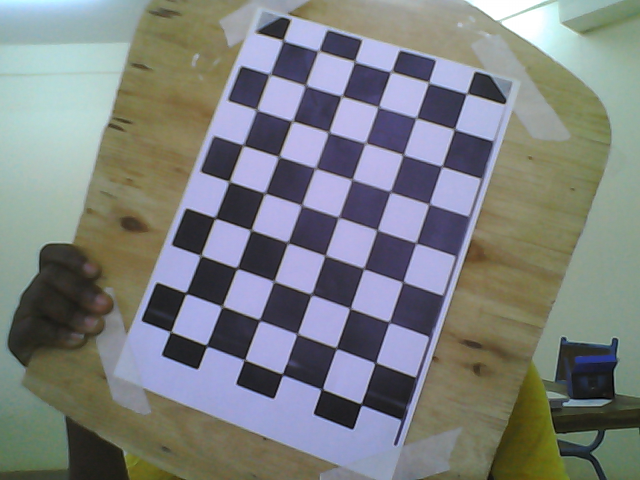
\includegraphics[scale=0.70]{image/img1.png}
	%\end{figure}
%\hspace{2 cm}
%	\begin{figure}
%			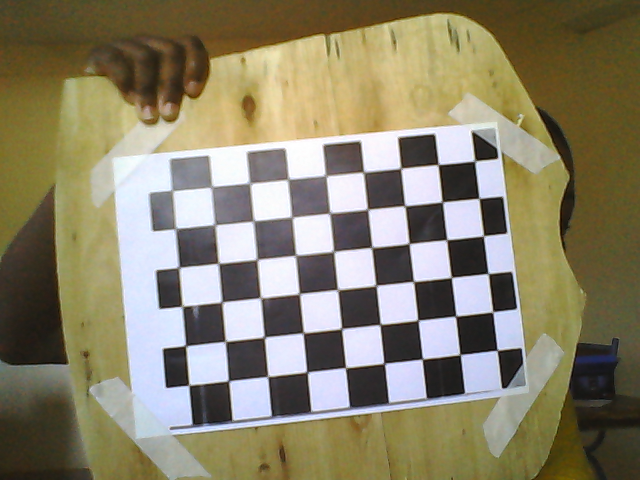
\includegraphics[scale=0.70]{image/img2.png}
%	\end{figure}

	%\decoRule
%	\caption[Image du damier ]{Image du damier utilisé.}
	%\label{Image du damier}
%\end{figure}

%\section{Première partie: Mesure avec le bois}
%\section{Deuxième partie: Intervention d'humain }







